\chapter{Theoretical Background}
\label{chap:theoretical-background}

This chapter establishes the theoretical foundation necessary for understanding the design and implementation of the Variant Management and Parametrization (VMAP) database system. It begins with an overview of database systems and their types, followed by an examination of database design methodologies, including entity-relationship modeling. The chapter then explores software development models relevant to automotive parameter management, particularly the V-Model that underpins the release management approach. Finally, it discusses role-based access control systems, version control concepts, and temporal database management, which are critical for the parameter versioning requirements of automotive software development.

\section{Database Management Systems}
\label{sec:database-management-systems}

Database management systems (DBMS) serve as the foundation for structured information storage and retrieval. They provide mechanisms for storing, organizing, and accessing data while ensuring integrity, security, and concurrent access \cite{elmasri2015fundamentals}. The choice of database system significantly impacts the design and capabilities of applications built upon it, making it a critical architectural decision for any information system. The basic division is made into two categories: relational and non-relational.

\subsection{Relational Database Management Systems}
\label{subsec:relational-database-management-systems}

Relational Database Management Systems (RDBMS) organize data into structured tables composed of rows and columns, based on the relational model proposed by E.F. Codd in 1970 \cite{codd1970relational}. The relational model establishes a mathematical foundation for representing data as relations (tables) with well-defined operations for data manipulation. This approach has dominated database technology for decades due to its solid theoretical foundation and practical advantages for structured data management.

In relational databases, tables adhere to predefined schemas that specify the structure, data types, and constraints applicable to the data. Each table typically includes a primary key that uniquely identifies each row, while foreign keys establish relationships between tables, implementing the referential integrity that ensures consistency across related data. Figure \ref{fig:relational-schema} illustrates a simple relational schema.

\begin{figure}[ht]
    \centering
    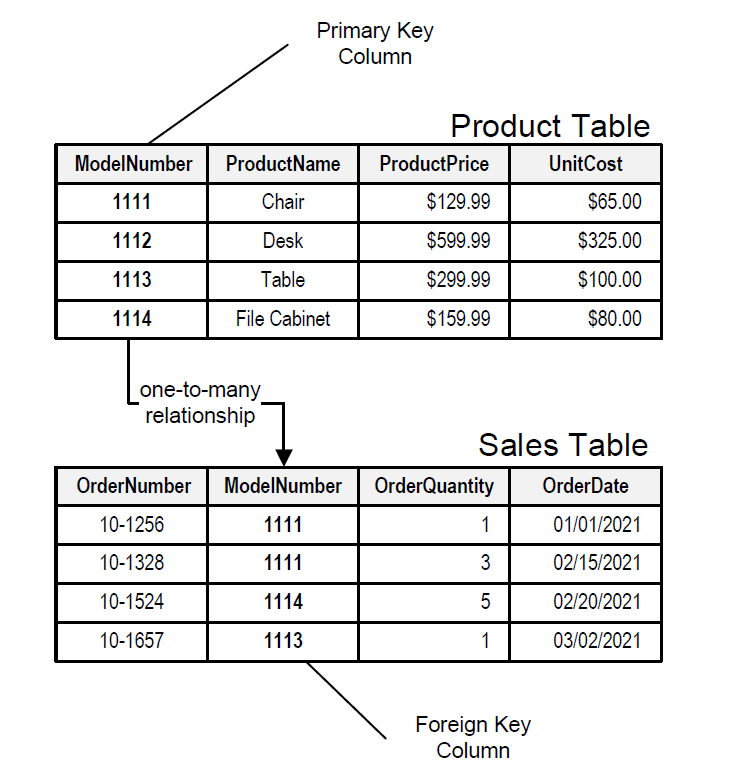
\includegraphics[width=0.85\textwidth]{figures/relational_schema.png}
    \caption{Example of a Relational Schema \cite{noah2024relational}}
    \label{fig:relational-schema}
\end{figure}

A key strength of relational databases is their adherence to ACID properties (Atomicity, Consistency, Isolation, Durability), which ensure reliable transaction processing. Atomicity guarantees that transactions are treated as indivisible units that either complete entirely or have no effect. Consistency ensures that transactions maintain database integrity by transforming the database from one valid state to another. Isolation prevents interference between concurrent transactions, making them appear as if executed sequentially. Durability ensures that committed transactions persist even after system failures.

ACID compliance makes relational databases particularly suitable for applications where data integrity and consistency are paramount, such as financial systems, healthcare records, and automotive parameter management where configuration errors could lead to safety issues \cite{staron2021automotive}. For the VMAP system, where incorrect parameter values could potentially affect vehicle safety and performance, the strong consistency guarantees of relational databases provide essential safeguards against data corruption or inconsistency.

\subsection{Non-Relational Database Systems}
\label{subsec:non-relational-database-systems}

Non-relational databases, often referred to as NoSQL (Not Only SQL) databases, emerged as alternatives to the relational model, particularly for use cases involving large-scale distributed systems, unstructured data, or schema flexibility requirements. Unlike relational databases, NoSQL systems typically sacrifice some aspects of ACID compliance in favor of scalability, flexibility, and performance characteristics suited to specific application domains \cite{bhattacherjee2015principles}.

NoSQL databases can be categorized into several types based on their data models. Document databases such as MongoDB and CouchDB store semi-structured data as documents, typically in formats like JSON or XML, allowing flexible schema evolution. Key-value stores like Redis and DynamoDB provide simple data access through key-based lookups, optimized for high-throughput operations. Column-family stores such as Cassandra and HBase organize data in column families for efficient storage and retrieval of large datasets. Graph databases like Neo4j and Amazon Neptune optimize the storage and traversal of highly connected data structures.

\begin{figure}[ht]
    \centering
    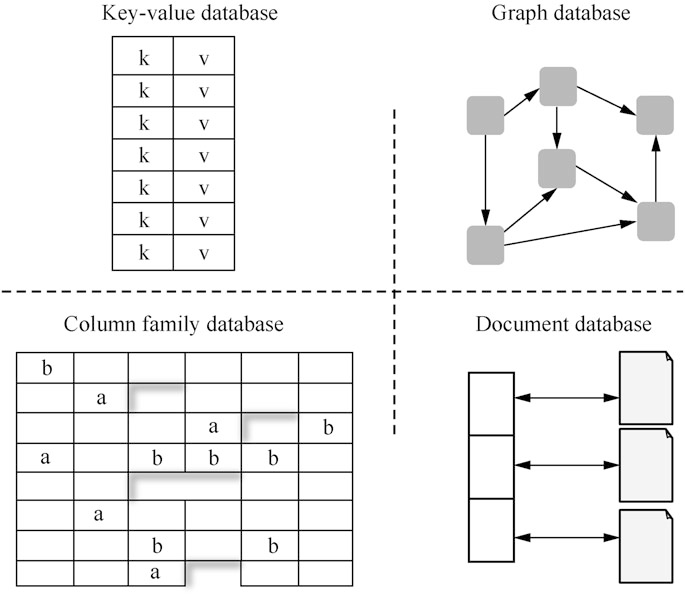
\includegraphics[width=0.85\textwidth]{figures/nosql_types.png}
    \caption{Major Types of NoSQL Databases \cite{gaussdbdatabase}}
    \label{fig:nosql-types}
\end{figure}

Many NoSQL systems follow the BASE principle (Basically Available, Soft state, Eventually consistent) rather than ACID, prioritizing availability and partition tolerance over immediate consistency. This approach aligns with the CAP theorem proposed by Brewer \cite{brewer2000robust}, which states that distributed systems can guarantee at most two of the following three properties: Consistency, Availability, and Partition tolerance.

While NoSQL databases excel in specific domains such as high-volume web applications, real-time analytics, and social networks, they present challenges for applications requiring complex transactions, strict data integrity, or sophisticated query capabilities across related entities \cite{kleppmann2017conflict}. For automotive parameter management, where data integrity and complex relationships between parameters, variants, and configurations are essential, the trade-offs presented by NoSQL systems make them less suitable than relational databases. The potential for eventual consistency rather than immediate consistency could lead to incorrect parameter configurations being used during development or testing, creating significant risks for vehicle performance and safety.

Additionally, the hierarchical nature of automotive electronic systems, with ECUs containing modules, PIDs, and parameters in well-defined relationships, aligns naturally with the relational model's approach to representing structured data and relationships. The ability to enforce these relationships through foreign key constraints provides important safeguards against data inconsistency that would be more difficult to implement in many NoSQL systems.

\subsection{Database Normalization}
\label{subsec:database-normalization}

Database normalization is a systematic approach to reduce data redundancy and improve data integrity in relational database design. Developed by E.F. Codd alongside the relational model, normalization organizes data into progressively more structured forms through a series of normal forms \cite{codd1970relational}. Each normal form addresses specific types of anomalies that could occur in database operations.

First Normal Form (1NF) eliminates repeating groups by ensuring atomic values in each column. Second Normal Form (2NF) removes partial dependencies on primary keys. Third Normal Form (3NF) eliminates transitive dependencies between non-key attributes. Boyce-Codd Normal Form (BCNF) addresses anomalies not resolved by 3NF in cases with multiple candidate keys. Fourth and Fifth Normal Forms (4NF, 5NF) address multi-valued dependencies and join dependencies, respectively.

Normalization significantly reduces data redundancy, thereby minimizing update anomalies and improving data integrity. However, for complex applications like automotive parameter management, a balance must be struck between full normalization and performance considerations. Denormalization—the deliberate introduction of controlled redundancy—may be employed to optimize specific query patterns while maintaining overall data integrity \cite{elmasri2015fundamentals}.

For the VMAP system, normalization principles guide the design of core entities and relationships, while strategic denormalization is applied to support performance-critical operations such as parameter retrieval and variant resolution. This balanced approach ensures data integrity while providing the performance characteristics needed for interactive use in automotive development environments.

\section{Database Design Methodologies}
\label{sec:database-design-methodologies}

Effective database design is crucial for ensuring that a database system meets its functional requirements while maintaining performance, scalability, and maintainability. Several methodologies have been developed to guide the database design process, each with its own strengths and applicability to different problem domains.

\subsection{Entity-Relationship Modeling}
\label{subsec:entity-relationship-modeling}

Entity-Relationship (ER) modeling is a conceptual approach to database design that focuses on identifying the entities, attributes, and relationships in a domain. Proposed by Peter Chen in 1976 \cite{chen1976entity}, ER modeling provides a graphical notation for representing database structures that is both intuitive for stakeholders and precise enough for technical implementation.

The key components of ER modeling include entities, which represent distinct objects or concepts in the domain (e.g., ECUs, Modules, Parameters); attributes, which describe properties of entities (e.g., name, description, value); relationships, which depict associations between entities, specifying cardinality (e.g., one-to-one, one-to-many, many-to-many); and constraints, which define rules that data must satisfy (e.g., uniqueness, referential integrity).

\begin{figure}[ht]
    \centering
    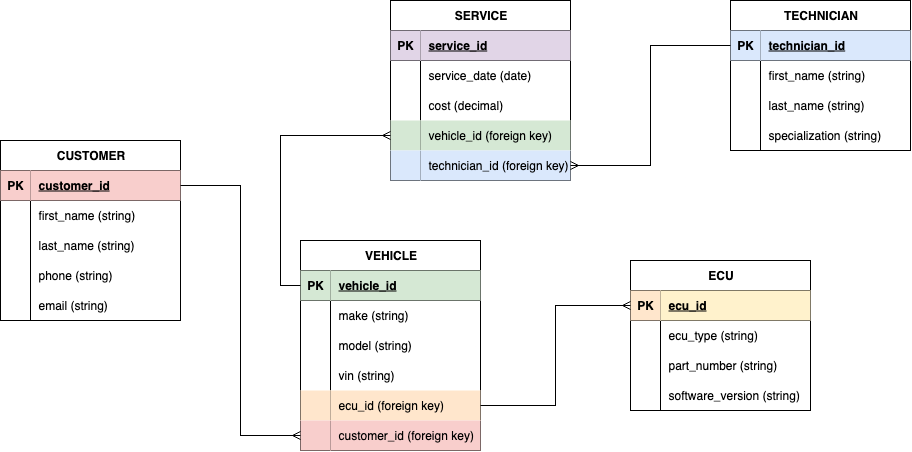
\includegraphics[width=0.85\textwidth]{figures/er_diagram.png}
    \caption{Entity-Relationship Diagram for Core VMAP Entities \cite{RelationalData}}
    \label{fig:er-diagram}
\end{figure}

ER modeling provides several advantages for database design: it focuses on domain understanding before implementation details, facilitates communication between technical and non-technical stakeholders, and provides a clear pathway to logical and physical database design \cite{elmasri2015fundamentals}. For complex domains like automotive parameter management, where intricate relationships exist between different entities, ER modeling offers a structured approach to capturing and representing these complexities.

The VMAP system utilizes ER modeling as the primary approach for database design, providing a conceptual framework that captures the complex relationships between ECUs, modules, PIDs, parameters, variants, and segments, as well as the temporal relationships introduced by the phase-based versioning model.

\subsection{Object-Relational Mapping}
\label{subsec:object-relational-mapping}

Object-Relational Mapping (ORM) bridges the gap between object-oriented programming and relational database systems by mapping objects in code to relational database structures. This approach addresses the "impedance mismatch" between object-oriented design and relational data models, allowing developers to work with database entities using the object-oriented paradigm \cite{ireland2009classification}.

ORM frameworks provide several benefits for application development: they reduce boilerplate code for database operations, abstract database-specific syntax, support database-agnostic application development, and integrate with application-level validation and business logic. However, ORM approaches can introduce performance overhead and may obscure complex query optimizations. For performance-critical applications like automotive parameter management, a balanced approach combining ORM for routine operations with direct SQL for complex queries often provides the best results \cite{ireland2009classification}.

The VMAP system employs a hybrid approach, using the Dapper micro-ORM framework to balance the convenience of object mapping with the performance advantages of direct SQL queries for complex operations involving parameter versioning and variant resolution. This approach provides the benefits of object-oriented development while maintaining the performance characteristics needed for a responsive parameter management system.

\section{Software Development Methodologies for Automotive Systems}
\label{sec:software-development-methodologies}

The development of automotive software systems follows specialized methodologies that address the unique challenges of safety-critical embedded systems. These methodologies incorporate aspects of systems engineering, software engineering, and quality assurance to ensure that automotive software meets stringent requirements for reliability, safety, and compliance.

% \subsection{V-Model for Automotive Development}
% \label{subsec:v-model}

% The V-Model is widely adopted in automotive software development due to its emphasis on validation and verification at each development stage \cite{broy2006challenges}. This model establishes a systematic approach to development, where each phase on the descending side of the "V" has a corresponding validation activity on the ascending side, as illustrated in Figure \ref{fig:v-model}.

% \begin{figure}[ht]
%     \centering
%     %\includegraphics[width=0.85\textwidth]{figures/v_model.png}
%     \caption{V-Model for Automotive Software Development}
%     \label{fig:v-model}
% \end{figure}

% The V-Model includes phases such as requirements analysis, system design, detailed design, implementation, component testing, integration testing, system testing, and acceptance testing. In automotive development, this model is often extended to include safety analysis, formal verification, and compliance verification steps. The structured nature of the V-Model aligns well with the parameter development process in automotive systems, where each parameter configuration must progress through defined stages of development, testing, and validation before release \cite{staron2021automotive}.

% The release phases in automotive parameter development (Phase1, Phase1, Phase1, Phase1) correspond to stages in the V-Model, providing a structured framework for parameter evolution throughout the development lifecycle. This alignment between the parameter versioning model and the overall development methodology ensures consistency in the development process and facilitates compliance with automotive standards such as ISO 26262 \cite{staron2021automotive}.

% The VMAP system's phase-based versioning approach directly supports this development model, enabling parameter configurations to progress through the defined development stages with appropriate controls and validation at each transition. This alignment between the database architecture and the automotive development methodology ensures that the system supports established development practices while providing the technical capabilities needed for effective parameter management.

\subsection{Use Case Driven Development}
\label{subsec:use-case-driven-development}

Use Case Driven Development focuses on defining system functionality from the perspective of user interactions. This approach begins with the identification of actors (users or external systems) and the definition of use cases that describe how these actors interact with the system to achieve specific goals \cite{jacobson2004use}.

\begin{figure}[ht]
    \centering
    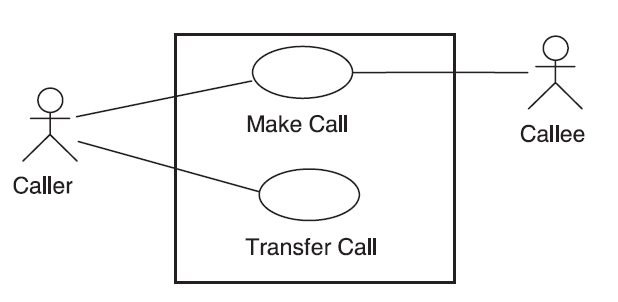
\includegraphics[width=0.85\textwidth]{figures/use_case_diagram.png}
    \caption{Use Case Diagram of switching system \cite{jacobson2004use}}
    \label{fig:use-case-diagram}
\end{figure}

Use cases provide several advantages for system development: they focus on user needs rather than technical implementation, establish a common understanding between stakeholders, provide a foundation for requirements validation and testing, and help identify system boundaries and external interfaces. In automotive parameter management, use cases help define the specific workflows for different user roles (Module Developers, Documentation Team, Administrators, Read-Only Users), ensuring that the system addresses the actual needs of development teams while maintaining appropriate access controls and security boundaries \cite{sandhu1998role}.

The VMAP system's database design is influenced by use case analysis, with database structures and operations aligned with the specific needs of different user roles and their interactions with parameter data. This alignment ensures that the database provides efficient support for common workflows while maintaining appropriate security boundaries and access controls.

\section{Access Control and Security Models}
\label{sec:access-control-security-models}

Access control is a critical aspect of database systems, particularly for automotive parameter management where different user roles have distinct responsibilities and permissions. Several models have been developed to address access control requirements, each with its own approach to defining and enforcing permissions.

\subsection{Role-Based Access Control}
\label{subsec:role-based-access-control}

Role-Based Access Control (RBAC) organizes access permissions around roles rather than individual users, simplifying security administration and aligning access rights with organizational structures \cite{sandhu1998role}. In RBAC, users are assigned to roles, and roles are granted permissions for specific operations on system resources.

The core components of RBAC include users (individuals who need access to system resources), roles (collections of permissions that correspond to job functions), permissions (defined operations on specific resources), and sessions (temporary bindings between users and their assigned roles).

\begin{figure}[ht]
    \centering
    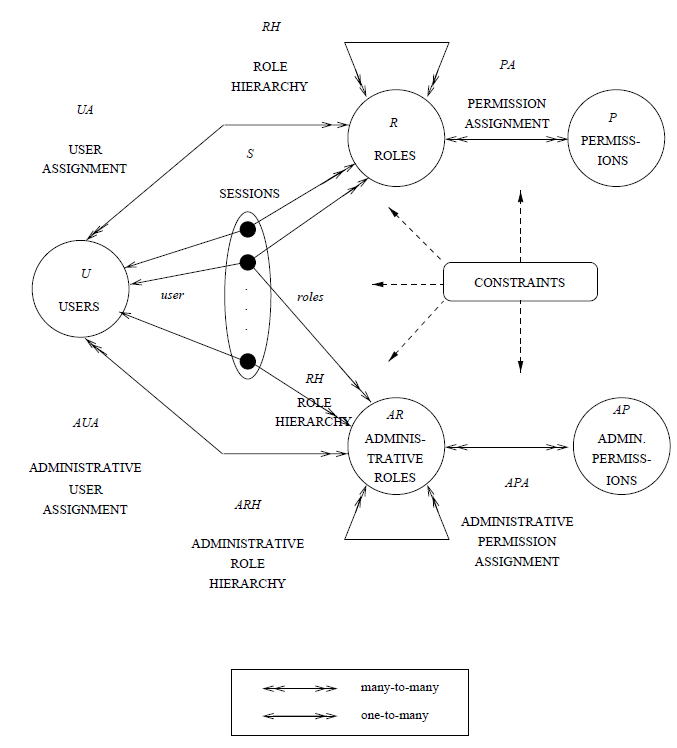
\includegraphics[width=0.85\textwidth]{figures/rbac_model.png}
    \caption{Role-Based Access Control Model \cite{sandhu1998role}}
    \label{fig:rbac-model}
\end{figure}

The separation between users and permissions through roles provides several advantages: it simplifies security administration, as permissions are managed at the role level; reduces the risk of permission errors, as roles are defined based on job functions; supports the principle of least privilege, giving users only the permissions needed for their responsibilities; and facilitates compliance with regulatory requirements through structured assignment of permissions.

For automotive parameter management, RBAC provides an effective framework for managing the complex access requirements of different user groups. By defining roles that align with specific responsibilities in the parameter development process (e.g., Module Developer, Documentation Specialist), the system can enforce appropriate access controls while supporting collaborative development activities \cite{ferraiolo2011policy}.

The VMAP system implements RBAC as the primary access control model, with roles defined for Module Developers, Documentation Team members, Administrators, and Read-Only Users, each with specific permissions aligned with their responsibilities in the parameter development process. This role-based approach provides a clear and manageable security model that supports the collaborative nature of automotive parameter development while maintaining appropriate access controls.

\subsection{Attribute-Based Access Control}
\label{subsec:attribute-based-access-control}

Attribute-Based Access Control (ABAC) extends beyond role-based approaches by making access decisions based on attributes of users, resources, actions, and environment \cite{hu2015implementing}. This more flexible approach allows fine-grained access control based on multiple factors rather than predefined roles.

ABAC components typically include subject attributes (properties of the user, such as department, job title, clearance level), resource attributes (properties of the accessed resource, such as module, classification, owner), action attributes (properties of the operation being performed), and environment attributes (contextual information such as time, location, system status).

ABAC offers greater flexibility than RBAC but requires more complex policy definition and evaluation. For systems with dynamic access requirements or where permissions depend on contextual factors, ABAC provides advantages over purely role-based approaches \cite{xu2014specification}. In automotive parameter management, a hybrid approach combining RBAC with attribute-based extensions often provides the best balance, using roles for general permission assignment while incorporating attribute-based rules for module-specific access control or phase-specific permissions \cite{sandhu1997arbac97}.

The VMAP system extends the basic RBAC model with attribute-based elements, particularly for module-specific access control. This hybrid approach allows Module Developers to be granted write access to specific modules rather than all modules, implementing the principle of least privilege while maintaining the overall role-based security structure. This combination provides both manageability and flexibility, addressing the specific security requirements of automotive parameter management.

\section{Version Control and Temporal Database Concepts}
\label{sec:version-control-temporal-concepts}

Version control is essential for managing the evolution of software artifacts, including database content. For automotive parameter management, where parameters evolve through multiple development phases and variants, sophisticated versioning approaches are required to maintain traceability and consistency.

\subsection{Traditional Version Control Systems}
\label{subsec:traditional-version-control}

Traditional Version Control Systems (VCS) focus on tracking changes to files over time, providing mechanisms for branching, merging, and maintaining change history \cite{tichy1985rcs}. These systems typically use either a centralized model (e.g., Subversion) or a distributed model (e.g., Git) for managing repositories.

Key features of traditional VCS include change tracking with commit history, branching and merging for parallel development, tagging for marking significant versions, and conflict detection and resolution mechanisms. While these systems excel at managing textual content like source code, they face limitations when dealing with structured data in databases. The file-centric nature of traditional VCS does not align well with the relational structure of databases, leading to challenges in tracking changes to individual records or maintaining relationships between related entities during version evolution \cite{bhattacherjee2015principles}.

For automotive parameter management, where complex relationships exist between parameters, variants, and configurations, specialized versioning approaches are needed that address the unique requirements of structured data evolution. The VMAP system addresses these requirements through a phase-based versioning model that explicitly represents development stages and their relationships, combined with comprehensive change tracking mechanisms that maintain a complete audit trail of parameter modifications.

\subsection{Temporal Database Concepts}
\label{subsec:temporal-database-concepts}

Temporal databases extend traditional database systems with explicit support for time-varying data, allowing queries based on time dimensions and maintaining historical states \cite{kulkarni2012temporal}. These systems typically support two time dimensions: valid time (when facts are true in the modeled reality) and transaction time (when facts are recorded in the database). Databases that support both dimensions are known as bi-temporal databases, providing a comprehensive framework for tracking both when changes occurred in the system and when they became effective in the real world \cite{bohlen2018database}.

\begin{figure}[ht]
    \centering
    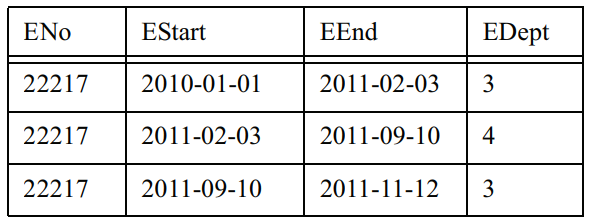
\includegraphics[width=0.85\textwidth]{figures/temporal_database.png}
    \caption{Temporal Database Example \cite{kulkarni2012temporal}}
    \label{fig:temporal-database}
\end{figure}

Temporal database concepts provide several advantages for version management: automatic preservation of historical states, support for as-of-date queries across different time points, simplified auditing and compliance reporting, and consistent handling of time-based business rules. However, temporal databases also introduce complexities in schema design, query formulation, and performance optimization. For automotive parameter management, where versioning requirements align with specific development phases rather than continuous time, a domain-specific approach combining elements of temporal databases with phase-based versioning often provides the most effective solution \cite{bhattacherjee2015principles}.

The VMAP system adopts a hybrid approach to versioning, using explicit phase associations rather than temporal timestamps as the primary versioning dimension. This approach aligns more directly with the automotive development process, where parameters progress through discrete development phases rather than evolving continuously over time. The phase-based approach simplifies queries for specific development stages while maintaining the version history needed for traceability and compliance.

\subsection{Database Versioning Approaches}
\label{subsec:database-versioning-approaches}

Several approaches have been developed for managing database versioning, each with its own trade-offs in terms of complexity, query performance, and storage requirements. Schema versioning tracks changes to database structure through migration scripts or schema evolution mechanisms \cite{curino2009automating}. Tuple versioning maintains multiple versions of each row (tuple) with validity periods, supporting time-travel queries but potentially increasing storage requirements \cite{saracco2010matter}. Snapshot isolation creates complete copies of data at specific points in time, simplifying retrieval of historical states but increasing storage overhead \cite{bhattacherjee2015principles}. Change logging records all modifications in an audit trail, providing complete change history while minimizing storage overhead for unchanged data \cite{bhattacherjee2015principles}.

% \begin{figure}[ht]
%     \centering
%     %\includegraphics[width=0.85\textwidth]{figures/versioning_approaches.png}
%     \caption{Comparison of Database Versioning Approaches}
%     \label{fig:versioning-approaches}
% \end{figure}

For automotive parameter management, where parameters evolve through distinct development phases, a combination of these approaches often provides the most effective solution. The VMAP system implements a phase-based versioning approach with explicit association between parameters and development phases, supplemented by comprehensive change logging for auditability. This combined approach addresses the versioning requirements of automotive parameter management while maintaining acceptable performance characteristics \cite{broy2006challenges}.

The phase-based approach aligns directly with the automotive development process, making the version model more intuitive for users while simplifying common operations such as parameter retrieval and phase transition. The comprehensive change logging provides the detailed audit trail needed for compliance and traceability, recording who made each change, when it was made, and what was modified. This combination of phase-based versioning and detailed change logging provides the versioning capabilities needed for automotive parameter management while avoiding the complexity of full temporal database implementations.
